\documentclass[ignorenonframetext,]{beamer}
\setbeamertemplate{caption}[numbered]
\setbeamertemplate{caption label separator}{: }
\setbeamercolor{caption name}{fg=normal text.fg}
\beamertemplatenavigationsymbolsempty
\usepackage{lmodern}
\usepackage{amssymb,amsmath}
\usepackage{ifxetex,ifluatex}
\usepackage{fixltx2e} % provides \textsubscript
\ifnum 0\ifxetex 1\fi\ifluatex 1\fi=0 % if pdftex
  \usepackage[T1]{fontenc}
  \usepackage[utf8]{inputenc}
\else % if luatex or xelatex
  \ifxetex
    \usepackage{mathspec}
  \else
    \usepackage{fontspec}
  \fi
  \defaultfontfeatures{Ligatures=TeX,Scale=MatchLowercase}
\fi
% use upquote if available, for straight quotes in verbatim environments
\IfFileExists{upquote.sty}{\usepackage{upquote}}{}
% use microtype if available
\IfFileExists{microtype.sty}{%
\usepackage{microtype}
\UseMicrotypeSet[protrusion]{basicmath} % disable protrusion for tt fonts
}{}
\newif\ifbibliography
\hypersetup{
            pdftitle={Clase 4 de Mayo},
            pdfauthor={Mariano Dominguez},
            pdfborder={0 0 0},
            breaklinks=true}
\urlstyle{same}  % don't use monospace font for urls
\usepackage{color}
\usepackage{fancyvrb}
\newcommand{\VerbBar}{|}
\newcommand{\VERB}{\Verb[commandchars=\\\{\}]}
\DefineVerbatimEnvironment{Highlighting}{Verbatim}{commandchars=\\\{\}}
% Add ',fontsize=\small' for more characters per line
\usepackage{framed}
\definecolor{shadecolor}{RGB}{248,248,248}
\newenvironment{Shaded}{\begin{snugshade}}{\end{snugshade}}
\newcommand{\KeywordTok}[1]{\textcolor[rgb]{0.13,0.29,0.53}{\textbf{#1}}}
\newcommand{\DataTypeTok}[1]{\textcolor[rgb]{0.13,0.29,0.53}{#1}}
\newcommand{\DecValTok}[1]{\textcolor[rgb]{0.00,0.00,0.81}{#1}}
\newcommand{\BaseNTok}[1]{\textcolor[rgb]{0.00,0.00,0.81}{#1}}
\newcommand{\FloatTok}[1]{\textcolor[rgb]{0.00,0.00,0.81}{#1}}
\newcommand{\ConstantTok}[1]{\textcolor[rgb]{0.00,0.00,0.00}{#1}}
\newcommand{\CharTok}[1]{\textcolor[rgb]{0.31,0.60,0.02}{#1}}
\newcommand{\SpecialCharTok}[1]{\textcolor[rgb]{0.00,0.00,0.00}{#1}}
\newcommand{\StringTok}[1]{\textcolor[rgb]{0.31,0.60,0.02}{#1}}
\newcommand{\VerbatimStringTok}[1]{\textcolor[rgb]{0.31,0.60,0.02}{#1}}
\newcommand{\SpecialStringTok}[1]{\textcolor[rgb]{0.31,0.60,0.02}{#1}}
\newcommand{\ImportTok}[1]{#1}
\newcommand{\CommentTok}[1]{\textcolor[rgb]{0.56,0.35,0.01}{\textit{#1}}}
\newcommand{\DocumentationTok}[1]{\textcolor[rgb]{0.56,0.35,0.01}{\textbf{\textit{#1}}}}
\newcommand{\AnnotationTok}[1]{\textcolor[rgb]{0.56,0.35,0.01}{\textbf{\textit{#1}}}}
\newcommand{\CommentVarTok}[1]{\textcolor[rgb]{0.56,0.35,0.01}{\textbf{\textit{#1}}}}
\newcommand{\OtherTok}[1]{\textcolor[rgb]{0.56,0.35,0.01}{#1}}
\newcommand{\FunctionTok}[1]{\textcolor[rgb]{0.00,0.00,0.00}{#1}}
\newcommand{\VariableTok}[1]{\textcolor[rgb]{0.00,0.00,0.00}{#1}}
\newcommand{\ControlFlowTok}[1]{\textcolor[rgb]{0.13,0.29,0.53}{\textbf{#1}}}
\newcommand{\OperatorTok}[1]{\textcolor[rgb]{0.81,0.36,0.00}{\textbf{#1}}}
\newcommand{\BuiltInTok}[1]{#1}
\newcommand{\ExtensionTok}[1]{#1}
\newcommand{\PreprocessorTok}[1]{\textcolor[rgb]{0.56,0.35,0.01}{\textit{#1}}}
\newcommand{\AttributeTok}[1]{\textcolor[rgb]{0.77,0.63,0.00}{#1}}
\newcommand{\RegionMarkerTok}[1]{#1}
\newcommand{\InformationTok}[1]{\textcolor[rgb]{0.56,0.35,0.01}{\textbf{\textit{#1}}}}
\newcommand{\WarningTok}[1]{\textcolor[rgb]{0.56,0.35,0.01}{\textbf{\textit{#1}}}}
\newcommand{\AlertTok}[1]{\textcolor[rgb]{0.94,0.16,0.16}{#1}}
\newcommand{\ErrorTok}[1]{\textcolor[rgb]{0.64,0.00,0.00}{\textbf{#1}}}
\newcommand{\NormalTok}[1]{#1}
\usepackage{graphicx,grffile}
\makeatletter
\def\maxwidth{\ifdim\Gin@nat@width>\linewidth\linewidth\else\Gin@nat@width\fi}
\def\maxheight{\ifdim\Gin@nat@height>\textheight0.8\textheight\else\Gin@nat@height\fi}
\makeatother
% Scale images if necessary, so that they will not overflow the page
% margins by default, and it is still possible to overwrite the defaults
% using explicit options in \includegraphics[width, height, ...]{}
\setkeys{Gin}{width=\maxwidth,height=\maxheight,keepaspectratio}

% Prevent slide breaks in the middle of a paragraph:
\widowpenalties 1 10000
\raggedbottom

\AtBeginPart{
  \let\insertpartnumber\relax
  \let\partname\relax
  \frame{\partpage}
}
\AtBeginSection{
  \ifbibliography
  \else
    \let\insertsectionnumber\relax
    \let\sectionname\relax
    \frame{\sectionpage}
  \fi
}
\AtBeginSubsection{
  \let\insertsubsectionnumber\relax
  \let\subsectionname\relax
  \frame{\subsectionpage}
}

\setlength{\parindent}{0pt}
\setlength{\parskip}{6pt plus 2pt minus 1pt}
\setlength{\emergencystretch}{3em}  % prevent overfull lines
\providecommand{\tightlist}{%
  \setlength{\itemsep}{0pt}\setlength{\parskip}{0pt}}
\setcounter{secnumdepth}{0}

\title{Clase 4 de Mayo}
\author{Mariano Dominguez}
\date{April 24, 2018}

\begin{document}
\frame{\titlepage}

\begin{frame}{Análisis exploratorio y curación de datos}

\begin{itemize}
\tightlist
\item
  Mariano Dominguez @ IATE-OAC-UNC \& CONICET
\item
  Edgardo Hames @ Bitlogic
\item
  Gabriel Miretti @ Bitlogic
\end{itemize}

\begin{figure}
\centering

\includegraphics{./logos-diplomatura-3.png}
\caption{Diplodatos @ FaMAF}
\end{figure}

\end{frame}

\begin{frame}{Paradigmas cientificos clasicos:}

Siglos atras la ciencia era \textbf{empirica}, describiendo los procesos
naturales.

\begin{figure}
\centering
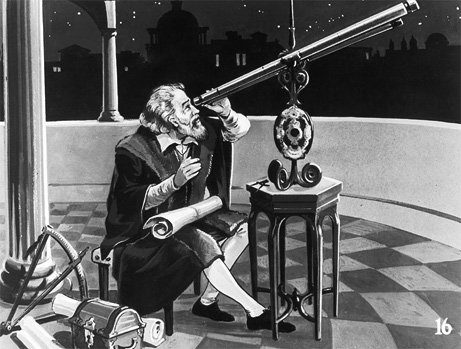
\includegraphics[width=0.30000\textwidth]{./13693233.jpg}
\caption{Galileo observando con un telescopio}
\end{figure}

luego se desarrollaron modelos \textbf{teoricos} matematicos,
generalizaciones

\begin{figure}
\centering
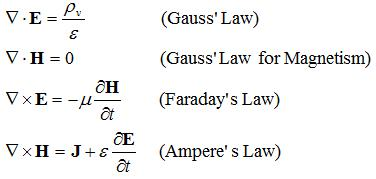
\includegraphics[width=0.30000\textwidth]{./maxwellseq.jpg}
\caption{Newton, Maxwell, Einstein, Dirac eqs}
\end{figure}

\end{frame}

\begin{frame}{Astronomia (u otra ciencia) Computacional}

En las ultimas decadas se han simulando fenomenos complejos.

\begin{figure}
\centering
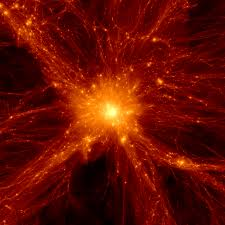
\includegraphics[width=0.40000\textwidth]{lcdm.jpeg}
\caption{Simulacion cosmologica LCDM}
\end{figure}

\end{frame}

\begin{frame}{El cuarto paradigma en ciencia:}

Hoy en dia la exploracion de datos (eScience) unifica la teoria, los
experimentos y las simulaciones.

-- Datos capturados por instrumentos o generados por una simulacion. --
Procesados por complejos pipelines de software. -- Cientifico analiza
bases de datos utilizando tecnicas estadisticas.

\begin{figure}
\centering
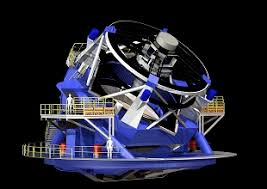
\includegraphics[width=0.30000\textwidth]{lsst.jpeg}
\caption{LSST telescopio y camara}
\end{figure}

\url{http://www.astro.caltech.edu/~george/aybi199/4th_paradigm_book_complete_lr.pdf}

\end{frame}

\begin{frame}{Por que (no) R? es FLOSS!}

Introduccion al lenguaje estadistico R \url{http://r-project.org} y CRAN
\url{http://cran.r-project.org/} : R consiste en una colleccion de
software con una importante variedad de paquetes para analisis de datos,
matematica aplicada, estadistica , graficos y diferentes utilidades. Los
paquetes extras en CRAN son suministrados por individuos o comunidades
de expertos en biologia, economia, geologia y otros campos (ver
\url{https://www.jstatsoft.org/index} ).

Existe una linda IDE: RStudio \url{https://www.rstudio.com/} y una muy
buena biblioteca para graficos ggplot2 (now ggviz). Tambien existen
diversas galeria de graficos en R y recientemente se ha establecido el
consorcio R: \url{https://www.r-consortium.org/} (Microsoft compro
Revolution, ver tambien h2o).

Se ha realizado un considerable esfuerzo para conectar R con otros
programas, lenguajes y sistemas estadisticos. Scripts en R pueden correr
facilmente desde la consola, pero mas esfuerzo es necesario para correr
programas en otros lenguajes. R se conecta con C, C++, FORTRAN, JaVa,
JavaScript, Matlab, Python, Perl, XLisp y Ruby. En algunos casos, las
interfaces son bidireccionales permitiendo el interambio de variables.
*** \#\# R Markdown

Esta es una presentacion en R Markdown. Markdown es un formato de
sintaxis simple para crear documentos HTML, PDF y MS Word. Por mas
detalles de comom utilizar R Markdown ver
\url{http://rmarkdown.rstudio.com}.

Cuando se clickea el boton \textbf{Knit}, un documento es generado que
incluye el contenido asi como los outputs de de los chuncks de codigos R
embebidos en el documento ver
\url{https://legacy.gitbook.com/book/bids/the-practice-of-reproducible-research/details}
y \url{https://arxiv.org/abs/1605.04339}.

\textbf{Shiny} is un paquete de R que permite constriur apps
interactivos directamente en R Markdown, webpages o cosntruir
dashboards. Ademas se pueden extender los Shiny apss con temas CSS,
htmlwidgets y herramientas de JavaScript
\url{https://shiny.rstudio.com/galley} .

\end{frame}

\begin{frame}[fragile]{Estadistica con R}

Una nocion basica es la de una muestra aleatoria.

E R es posible simular facilmente esta situacion con la funcion
\textbf{sample}. Si por ejemplo quiero elegir cinco numero aleatorios
entre 1 y 40, escribo:

\begin{verbatim}
## [1] 24  5 12  1 32
\end{verbatim}

Muestrear con reeemplazo es adecuado para modelar monedas o dados. Por
ejemplo para simular arrojar diez monedas podemos escribir:

\begin{verbatim}
##  [1] "H" "T" "H" "H" "T" "T" "T" "H" "T" "T"
\end{verbatim}

Tambien se puede simular datos con diferentes probabilidades de cada
resultado, (por ejemplo tener una tasa de exitos del 90\%) utilizando el
argumento prob in sample:

\begin{verbatim}
##  [1] "succ" "succ" "succ" "succ" "succ" "succ" "succ" "succ" "succ" "succ"
\end{verbatim}

\end{frame}

\begin{frame}{Distribuciones discretas en R:}

cuando las variables solo pueden tomar solamente valores finitos, es
preferible dibujar un digrama de alfileres (pin), aqui podemos observar
la distribucion binomial con n=50 y p=0.33.

\includegraphics{class1_files/figure-beamer/unnamed-chunk-4-1.pdf}

\end{frame}

\begin{frame}[fragile]{Numeros Aleatorios:}

En general suena contradictorio generar numeros aleatorios en una
computadora dado que se supone que sus resultados son predecibles y
reproducibles. Lo que en realidad es posible es generar secuencias de
numeros pseudo aleatorios, que para todos los efectos practicos se
comportan como si fueran aleatorios. Ver sobre LCGs,
\url{http://www.aaronschlegel.com/series/random-number-generation/}

En estadistica se utilizan para crear conjuntos de datos simulados para
estudiar los efectos de los algoritmos. El uso de funciones que generan
numeros aleatorios es simple, por ejemplo numeros que siguen una
distribucion normal:

\begin{verbatim}
## [1] -0.1850562
\end{verbatim}

\begin{verbatim}
## [1] 1.002957
\end{verbatim}

\begin{verbatim}
##         0%        25%        50%        75%       100% 
## -2.5330586 -0.8201091 -0.2844535  0.4053724  2.4728409
\end{verbatim}

\end{frame}

\begin{frame}[fragile]

\begin{block}{Distribution uniforme}

El generador basico en R es runif, cuya entrada es el numero de valores
a ser generados.

\begin{verbatim}
##  [1] 3.082045 4.037753 4.291460 4.159930 2.265714 4.971483 2.168713
##  [8] 4.769044 3.769811 3.699897
\end{verbatim}

Veamos como funciona:

\includegraphics{class1_files/figure-beamer/unnamed-chunk-7-1.pdf}

\end{block}

\end{frame}

\begin{frame}[fragile]

\begin{block}{Guardando las semillas.}

runif no implica aleatoridad per se. runif(Nsim) es calcular una
secuencia deterministica basada en un numero aleatorio inicial
(semilla).

\begin{Shaded}
\begin{Highlighting}[]
\KeywordTok{set.seed}\NormalTok{(}\DecValTok{1}\NormalTok{)}
\KeywordTok{runif}\NormalTok{(}\DecValTok{5}\NormalTok{)}
\end{Highlighting}
\end{Shaded}

\begin{verbatim}
## [1] 0.2655087 0.3721239 0.5728534 0.9082078 0.2016819
\end{verbatim}

\begin{Shaded}
\begin{Highlighting}[]
\KeywordTok{set.seed}\NormalTok{(}\DecValTok{1}\NormalTok{)}
\KeywordTok{runif}\NormalTok{(}\DecValTok{5}\NormalTok{)}
\end{Highlighting}
\end{Shaded}

\begin{verbatim}
## [1] 0.2655087 0.3721239 0.5728534 0.9082078 0.2016819
\end{verbatim}

\begin{Shaded}
\begin{Highlighting}[]
\KeywordTok{set.seed}\NormalTok{(}\DecValTok{2}\NormalTok{)}
\KeywordTok{runif}\NormalTok{(}\DecValTok{5}\NormalTok{)}
\end{Highlighting}
\end{Shaded}

\begin{verbatim}
## [1] 0.1848823 0.7023740 0.5733263 0.1680519 0.9438393
\end{verbatim}

\end{block}

\end{frame}

\begin{frame}

\begin{block}{La transformacion Inversa del CDF:}

Existe una transformacion simple, que nos permite transformar cualquier
variable aleatoria en una uniforme y mas importante viceversa.

Por ejemplo si \(x\) esta dada por una densidad de probabilidad \(f\) y
una CDF \(F\) , entonces vale la relacion:
\(F(x)=\int_{-\infty}^{x} f(t) \delta t\) y si elegmimos \(U = F (X)\),
con \(U\) una variable aleatoria distribuida uniformemente.

Ejemplo: Si \(X \propto exp\), entonces \(F (x) = 1-e^{-x}\) .
Resolviendo para \(x\) en \(u = 1-e^{-x}\) nos da \(x = -log(1 - u)\).
Por lo tanto si \(u\) es uniforme, entonces \(X \propto exp\)

\includegraphics{class1_files/figure-beamer/unnamed-chunk-10-1.pdf}

\end{block}

\end{frame}

\begin{frame}[fragile]{Submuestras}

Los comandos subset(), which() and ifelse() son probablemente los mas
utilizados en R. Una manera de filtrar elementos de un vector es
utilizar la funcion subset().

\begin{Shaded}
\begin{Highlighting}[]
\CommentTok{# create a vector}
\NormalTok{x <-}\StringTok{ }\KeywordTok{c}\NormalTok{(}\DecValTok{5}\NormalTok{,}\DecValTok{4}\OperatorTok{:}\DecValTok{8}\NormalTok{,}\DecValTok{12}\NormalTok{)}
\NormalTok{x}
\end{Highlighting}
\end{Shaded}

\begin{verbatim}
## [1]  5  4  5  6  7  8 12
\end{verbatim}

\begin{Shaded}
\begin{Highlighting}[]
\NormalTok{y <-}\StringTok{ }\KeywordTok{subset}\NormalTok{(x, x }\OperatorTok{<}\StringTok{ }\DecValTok{6}\NormalTok{)}
\NormalTok{y}
\end{Highlighting}
\end{Shaded}

\begin{verbatim}
## [1] 5 4 5
\end{verbatim}

\end{frame}

\begin{frame}[fragile]{Utilizando which()}

identifica la posicion del vector donde se cumple (is TRUE) la
condicion: Vea el siguiente ejemplo de como utilizarla:

\begin{Shaded}
\begin{Highlighting}[]
\CommentTok{# create a vector}
\NormalTok{z <-}\StringTok{ }\KeywordTok{c}\NormalTok{(}\DecValTok{6}\OperatorTok{:}\DecValTok{10}\NormalTok{, }\DecValTok{12}\NormalTok{, }\OperatorTok{-}\DecValTok{3}\NormalTok{)}
\NormalTok{z}
\end{Highlighting}
\end{Shaded}

\begin{verbatim}
## [1]  6  7  8  9 10 12 -3
\end{verbatim}

\begin{Shaded}
\begin{Highlighting}[]
\KeywordTok{which}\NormalTok{(z }\OperatorTok{>}\StringTok{ }\DecValTok{8}\NormalTok{)}
\end{Highlighting}
\end{Shaded}

\begin{verbatim}
## [1] 4 5 6
\end{verbatim}

\end{frame}

\begin{frame}[fragile]{Utilizando ifelse}

el comnado ifelse tiene dos opciones para ejecutar. Si la condicion es
TRUE se ejecuta la primera, si la condicion es FALSE se ejecuta la
segunda. La sintaxis es ifelse(condition, opcion1, opcion2). Un ejemplo
a continuacion.

\begin{Shaded}
\begin{Highlighting}[]
\CommentTok{# create a vector}
\NormalTok{x <-}\StringTok{ }\KeywordTok{c}\NormalTok{(}\OperatorTok{-}\DecValTok{2}\NormalTok{, }\DecValTok{5}\OperatorTok{:}\DecValTok{10}\NormalTok{, }\DecValTok{15}\NormalTok{)}
\NormalTok{x}
\end{Highlighting}
\end{Shaded}

\begin{verbatim}
## [1] -2  5  6  7  8  9 10 15
\end{verbatim}

\begin{Shaded}
\begin{Highlighting}[]
\CommentTok{# if values are < 7 will code those 1, else will become 0}
\KeywordTok{ifelse}\NormalTok{(x }\OperatorTok{<}\StringTok{ }\DecValTok{7}\NormalTok{, }\DecValTok{1}\NormalTok{, }\DecValTok{0}\NormalTok{)}
\end{Highlighting}
\end{Shaded}

\begin{verbatim}
## [1] 1 1 1 0 0 0 0 0
\end{verbatim}

\begin{Shaded}
\begin{Highlighting}[]
\CommentTok{# also you can do this}
\KeywordTok{ifelse}\NormalTok{(x }\OperatorTok{<}\StringTok{ }\DecValTok{7}\NormalTok{, }\DecValTok{1}\NormalTok{, x)}
\end{Highlighting}
\end{Shaded}

\begin{verbatim}
## [1]  1  1  1  7  8  9 10 15
\end{verbatim}

\end{frame}

\begin{frame}[fragile]{Code the Matrix 1:}

Creamos una matriz x con numeros provenientes de una funcion normal. y
llamamos a sus elementos con x{[}fila,columna{]}.

\begin{Shaded}
\begin{Highlighting}[]
\CommentTok{# matrix with 12 random numbers in 4 rows}
\NormalTok{x <-}\StringTok{ }\KeywordTok{matrix}\NormalTok{(}\KeywordTok{rnorm}\NormalTok{(}\DecValTok{12}\NormalTok{), }\DataTypeTok{nrow=}\DecValTok{4}\NormalTok{)}
\NormalTok{x }
\end{Highlighting}
\end{Shaded}

\begin{verbatim}
##            [,1]       [,2]       [,3]
## [1,]  1.2891946 -1.9527802 -0.0692199
## [2,]  0.5955489 -0.3774369  0.1197222
## [3,]  1.1870120  0.4915441  0.9573790
## [4,] -0.1418306  0.1169809 -0.3900849
\end{verbatim}

\begin{Shaded}
\begin{Highlighting}[]
\CommentTok{# find the number in 3rd row and 2nd column}
\NormalTok{x[}\DecValTok{3}\NormalTok{,}\DecValTok{2}\NormalTok{]}
\end{Highlighting}
\end{Shaded}

\begin{verbatim}
## [1] 0.4915441
\end{verbatim}

\end{frame}

\begin{frame}[fragile]{Code the Matrix 2:}

tambien es posible referirse a una columna o fila u obtener las
dimensiones.

\begin{Shaded}
\begin{Highlighting}[]
\CommentTok{# show second columns}
\NormalTok{x[,}\DecValTok{2}\NormalTok{]}
\end{Highlighting}
\end{Shaded}

\begin{verbatim}
## [1] -1.9527802 -0.3774369  0.4915441  0.1169809
\end{verbatim}

\begin{Shaded}
\begin{Highlighting}[]
\CommentTok{# show forth row}
\NormalTok{x[}\DecValTok{4}\NormalTok{,]}
\end{Highlighting}
\end{Shaded}

\begin{verbatim}
## [1] -0.1418306  0.1169809 -0.3900849
\end{verbatim}

\begin{Shaded}
\begin{Highlighting}[]
\CommentTok{# find number or columns and rows in matrix}
\KeywordTok{dim}\NormalTok{(x)}
\end{Highlighting}
\end{Shaded}

\begin{verbatim}
## [1] 4 3
\end{verbatim}

\end{frame}

\begin{frame}[fragile]

\begin{block}{Utilizando lazos en R:}

Cada vez que alguna operacion debe ser repetida un lazo resulta util. De
acuerdo el manual de R, entre los comandos basicos de control de flujo,
las construcciones para lazos son: fort, while y repeat, con las
clausulas adicionales break y next.

Un ejemplo de un lazo simple:

\begin{verbatim}
## [1] "This loop calculates the square of the first 10 elements of\nvector u1"
\end{verbatim}

\begin{verbatim}
## [1] 3.326407
## [1] 0.9550669
## [1] 0.4375794
## [1] 0.007272402
## [1] 0.5649414
## [1] 0.1361074
## [1] 0.01092893
## [1] 0.1821844
## [1] 0.443898
## [1] 0.3556551
\end{verbatim}

\begin{verbatim}
## [1] 10
\end{verbatim}

Por lo que el bloque del lazo es contenido por \{\}.

\end{block}

\end{frame}

\begin{frame}[fragile]

\begin{block}{Lazos anidados}

Supongamos que queremos manipular una matriz poniendo sus elementos con
valores especificos:

\begin{verbatim}
##       [,1] [,2] [,3] [,4] [,5] [,6] [,7] [,8] [,9] [,10]
##  [1,]    1    2    3    4    5    6    7    8    9    10
##  [2,]    2    4    6    8   10   12   14   16   18    20
##  [3,]    3    6    9   12   15   18   21   24   27    30
##  [4,]    4    8   12   16   20   24   28   32   36    40
##  [5,]    5   10   15   20   25   30   35   40   45    50
##  [6,]    6   12   18   24   30   36   42   48   54    60
##  [7,]    7   14   21   28   35   42   49   56   63    70
##  [8,]    8   16   24   32   40   48   56   64   72    80
##  [9,]    9   18   27   36   45   54   63   72   81    90
## [10,]   10   20   30   40   50   60   70   80   90   100
\end{verbatim}

\end{block}

\end{frame}

\begin{frame}[fragile]

\begin{block}{Vectorizacion 1:}

es la operacion de convertir repetidas operaciones en numeros
(escalares) en operaciones en vectores o matrices. Muchos lazos pueden
hacerse implicitos con vectorizacion.

el ejemplo mas elemental es la adicion de dos vectores v1 y v2 en un
vector v3, lo que puede hacerse elemento por elemento con un lazo:

\begin{Shaded}
\begin{Highlighting}[]
\NormalTok{n=}\DecValTok{100}
\NormalTok{v1 <-}\StringTok{ }\KeywordTok{rnorm}\NormalTok{(n)}
\NormalTok{v2 <-}\StringTok{ }\KeywordTok{rnorm}\NormalTok{(n)  }
\NormalTok{v3 <-}\StringTok{ }\DecValTok{0}
\CommentTok{#  }
\ControlFlowTok{for}\NormalTok{ (i }\ControlFlowTok{in} \DecValTok{1}\OperatorTok{:}\NormalTok{n)}
\NormalTok{\{}
\NormalTok{v3[i] <-v1[i] }\OperatorTok{+}\StringTok{ }\NormalTok{v2[i]}
\NormalTok{\}}
\end{Highlighting}
\end{Shaded}

\end{block}

\end{frame}

\begin{frame}[fragile]

\begin{block}{Vectorizacion 2:}

o utilizando la forma vectorizada:

\begin{Shaded}
\begin{Highlighting}[]
\NormalTok{v3 =}\StringTok{ }\NormalTok{v1 }\OperatorTok{+}\StringTok{ }\NormalTok{v2}
\end{Highlighting}
\end{Shaded}

lo que permite utilizar eficientemente rutinas muy eficientes de algebra
lineal (BLAS)

Comparemos el tiempo de ejecucion entre ambas soluciones:

\begin{Shaded}
\begin{Highlighting}[]
\NormalTok{m=}\DecValTok{10}\NormalTok{; n=}\DecValTok{10}\NormalTok{;}
\NormalTok{mymat<-}\KeywordTok{replicate}\NormalTok{(m, }\KeywordTok{rnorm}\NormalTok{(n)) }\CommentTok{# create matrix of normal random numbers}
\NormalTok{mydframe=}\KeywordTok{data.frame}\NormalTok{(mymat) }\CommentTok{# transform into data frame}
\CommentTok{# measure loop execution}
\KeywordTok{system.time}\NormalTok{(}
\ControlFlowTok{for}\NormalTok{ (i }\ControlFlowTok{in} \DecValTok{1}\OperatorTok{:}\NormalTok{m) \{}
\ControlFlowTok{for}\NormalTok{ (j }\ControlFlowTok{in} \DecValTok{1}\OperatorTok{:}\NormalTok{n) \{}
\NormalTok{mydframe[i,j]<-mydframe[i,j] }\OperatorTok{+}\StringTok{ }\DecValTok{10}\OperatorTok{*}\KeywordTok{sin}\NormalTok{(}\FloatTok{0.75}\OperatorTok{*}\NormalTok{pi)}
\NormalTok{\}}
\NormalTok{\}}
\NormalTok{)}
\end{Highlighting}
\end{Shaded}

\begin{verbatim}
##    user  system elapsed 
##   0.012   0.000   0.012
\end{verbatim}

Ejercicio: Mida el tiempo en una version vectorizada.

\end{block}

\end{frame}

\begin{frame}

\begin{block}{La familia de instrucciones apply.}

Esta compuesta de funciones intrinsecamente vectorizada y esta compuesta
de funciones ({[}s,l,m,r, t,v{]}apply) para manipular datos en forma de
matrices en una forma repetitiva, evitando el uso explicito de lazos.
Las primeras tres son las mas utilizadas:

\begin{enumerate}
\def\labelenumi{\arabic{enumi}.}
\item
  apply permite aplicar una funcion a filas (primer indice) o columnas
  (segundo indice) de una matriz.
\item
  lapply permite aplicar una dada funcion a cada elemento de una lista.
\item
  sapply igual que la anterior, pero se obtiene un vector en lugar de
  una lista.
\end{enumerate}

\end{block}

\end{frame}

\begin{frame}[fragile]

\begin{Shaded}
\begin{Highlighting}[]
\NormalTok{#### elementary example of apply function}
\CommentTok{# define matrix mymat by replicating the sequence 1:5 for 4 times and transforming into a matrix}
\NormalTok{mymat<-}\KeywordTok{matrix}\NormalTok{(}\KeywordTok{rep}\NormalTok{(}\KeywordTok{seq}\NormalTok{(}\DecValTok{5}\NormalTok{), }\DecValTok{4}\NormalTok{), }\DataTypeTok{ncol =} \DecValTok{5}\NormalTok{)}
\CommentTok{# mymat sum on rows}
\KeywordTok{apply}\NormalTok{(mymat, }\DecValTok{1}\NormalTok{, sum)}
\end{Highlighting}
\end{Shaded}

\begin{verbatim}
## [1] 15 15 15 15
\end{verbatim}

\begin{Shaded}
\begin{Highlighting}[]
\CommentTok{# mymat sum on columns}
\KeywordTok{apply}\NormalTok{(mymat, }\DecValTok{2}\NormalTok{, sum)}
\end{Highlighting}
\end{Shaded}

\begin{verbatim}
## [1] 10 11 12 13 14
\end{verbatim}

\begin{Shaded}
\begin{Highlighting}[]
\CommentTok{# produce a summary column wise (for each column)}
\KeywordTok{apply}\NormalTok{(mymat, }\DecValTok{2}\NormalTok{, }\ControlFlowTok{function}\NormalTok{(x, y) }\KeywordTok{summary}\NormalTok{(mymat))}
\end{Highlighting}
\end{Shaded}

\begin{verbatim}
##       [,1]             [,2]             [,3]             [,4]            
##  [1,] "Min.   :1.00  " "Min.   :1.00  " "Min.   :1.00  " "Min.   :1.00  "
##  [2,] "1st Qu.:1.75  " "1st Qu.:1.75  " "1st Qu.:1.75  " "1st Qu.:1.75  "
##  [3,] "Median :2.50  " "Median :2.50  " "Median :2.50  " "Median :2.50  "
##  [4,] "Mean   :2.50  " "Mean   :2.50  " "Mean   :2.50  " "Mean   :2.50  "
##  [5,] "3rd Qu.:3.25  " "3rd Qu.:3.25  " "3rd Qu.:3.25  " "3rd Qu.:3.25  "
##  [6,] "Max.   :4.00  " "Max.   :4.00  " "Max.   :4.00  " "Max.   :4.00  "
##  [7,] "Min.   :1.00  " "Min.   :1.00  " "Min.   :1.00  " "Min.   :1.00  "
##  [8,] "1st Qu.:1.75  " "1st Qu.:1.75  " "1st Qu.:1.75  " "1st Qu.:1.75  "
##  [9,] "Median :2.50  " "Median :2.50  " "Median :2.50  " "Median :2.50  "
## [10,] "Mean   :2.75  " "Mean   :2.75  " "Mean   :2.75  " "Mean   :2.75  "
## [11,] "3rd Qu.:3.50  " "3rd Qu.:3.50  " "3rd Qu.:3.50  " "3rd Qu.:3.50  "
## [12,] "Max.   :5.00  " "Max.   :5.00  " "Max.   :5.00  " "Max.   :5.00  "
## [13,] "Min.   :1.00  " "Min.   :1.00  " "Min.   :1.00  " "Min.   :1.00  "
## [14,] "1st Qu.:1.75  " "1st Qu.:1.75  " "1st Qu.:1.75  " "1st Qu.:1.75  "
## [15,] "Median :3.00  " "Median :3.00  " "Median :3.00  " "Median :3.00  "
## [16,] "Mean   :3.00  " "Mean   :3.00  " "Mean   :3.00  " "Mean   :3.00  "
## [17,] "3rd Qu.:4.25  " "3rd Qu.:4.25  " "3rd Qu.:4.25  " "3rd Qu.:4.25  "
## [18,] "Max.   :5.00  " "Max.   :5.00  " "Max.   :5.00  " "Max.   :5.00  "
## [19,] "Min.   :1.00  " "Min.   :1.00  " "Min.   :1.00  " "Min.   :1.00  "
## [20,] "1st Qu.:2.50  " "1st Qu.:2.50  " "1st Qu.:2.50  " "1st Qu.:2.50  "
## [21,] "Median :3.50  " "Median :3.50  " "Median :3.50  " "Median :3.50  "
## [22,] "Mean   :3.25  " "Mean   :3.25  " "Mean   :3.25  " "Mean   :3.25  "
## [23,] "3rd Qu.:4.25  " "3rd Qu.:4.25  " "3rd Qu.:4.25  " "3rd Qu.:4.25  "
## [24,] "Max.   :5.00  " "Max.   :5.00  " "Max.   :5.00  " "Max.   :5.00  "
## [25,] "Min.   :2.00  " "Min.   :2.00  " "Min.   :2.00  " "Min.   :2.00  "
## [26,] "1st Qu.:2.75  " "1st Qu.:2.75  " "1st Qu.:2.75  " "1st Qu.:2.75  "
## [27,] "Median :3.50  " "Median :3.50  " "Median :3.50  " "Median :3.50  "
## [28,] "Mean   :3.50  " "Mean   :3.50  " "Mean   :3.50  " "Mean   :3.50  "
## [29,] "3rd Qu.:4.25  " "3rd Qu.:4.25  " "3rd Qu.:4.25  " "3rd Qu.:4.25  "
## [30,] "Max.   :5.00  " "Max.   :5.00  " "Max.   :5.00  " "Max.   :5.00  "
##       [,5]            
##  [1,] "Min.   :1.00  "
##  [2,] "1st Qu.:1.75  "
##  [3,] "Median :2.50  "
##  [4,] "Mean   :2.50  "
##  [5,] "3rd Qu.:3.25  "
##  [6,] "Max.   :4.00  "
##  [7,] "Min.   :1.00  "
##  [8,] "1st Qu.:1.75  "
##  [9,] "Median :2.50  "
## [10,] "Mean   :2.75  "
## [11,] "3rd Qu.:3.50  "
## [12,] "Max.   :5.00  "
## [13,] "Min.   :1.00  "
## [14,] "1st Qu.:1.75  "
## [15,] "Median :3.00  "
## [16,] "Mean   :3.00  "
## [17,] "3rd Qu.:4.25  "
## [18,] "Max.   :5.00  "
## [19,] "Min.   :1.00  "
## [20,] "1st Qu.:2.50  "
## [21,] "Median :3.50  "
## [22,] "Mean   :3.25  "
## [23,] "3rd Qu.:4.25  "
## [24,] "Max.   :5.00  "
## [25,] "Min.   :2.00  "
## [26,] "1st Qu.:2.75  "
## [27,] "Median :3.50  "
## [28,] "Mean   :3.50  "
## [29,] "3rd Qu.:4.25  "
## [30,] "Max.   :5.00  "
\end{verbatim}

\end{frame}

\begin{frame}[fragile]{Importando y exportando datos.}

Los datos en R pueden guardarse como archivos .Rdata con la funcion
save. Que luego pueden leerse en R con load.

\begin{Shaded}
\begin{Highlighting}[]
\NormalTok{a <-}\StringTok{ }\DecValTok{1}\OperatorTok{:}\DecValTok{10}
\KeywordTok{save}\NormalTok{(a, }\DataTypeTok{file =} \StringTok{"Data.Rdata"}\NormalTok{)}
\KeywordTok{rm}\NormalTok{(a)}
\KeywordTok{load}\NormalTok{(}\StringTok{"Data.Rdata"}\NormalTok{)}
\KeywordTok{print}\NormalTok{(a)}
\end{Highlighting}
\end{Shaded}

\begin{verbatim}
##  [1]  1  2  3  4  5  6  7  8  9 10
\end{verbatim}

\end{frame}

\begin{frame}[fragile]{Presentando los Data Frames:}

El siguiente ejemplo crea un dataframe a y lo guarda como un archivo CSV
con write.cvs. Luego el dataframe is cargado desde el archivo a una
variable b con read.cvs.

\begin{Shaded}
\begin{Highlighting}[]
\NormalTok{var1 <-}\StringTok{ }\DecValTok{1}\OperatorTok{:}\DecValTok{5}
\NormalTok{var2 <-}\StringTok{ }\NormalTok{(}\DecValTok{1}\OperatorTok{:}\DecValTok{5}\NormalTok{) }\OperatorTok{/}\StringTok{ }\DecValTok{10}
\NormalTok{var3 <-}\StringTok{ }\KeywordTok{c}\NormalTok{(}\StringTok{"Diplo"}\NormalTok{, }\StringTok{"Datos"}\NormalTok{, }\StringTok{"en"}\NormalTok{, }\StringTok{"FaMAF"}\NormalTok{, }\StringTok{"@UNC"}\NormalTok{)}
\NormalTok{a <-}\StringTok{ }\KeywordTok{data.frame}\NormalTok{(var1, var2, var3)}
\KeywordTok{names}\NormalTok{(a) <-}\StringTok{ }\KeywordTok{c}\NormalTok{(}\StringTok{"VariableInt"}\NormalTok{, }\StringTok{"VariableReal"}\NormalTok{, }\StringTok{"VariableChar"}\NormalTok{)}
\KeywordTok{write.csv}\NormalTok{(a, }\StringTok{"Data.csv"}\NormalTok{, }\DataTypeTok{row.names =} \OtherTok{FALSE}\NormalTok{)}
 \CommentTok{#rm(a)}
\NormalTok{b <-}\StringTok{ }\KeywordTok{read.csv}\NormalTok{(}\StringTok{"Data.csv"}\NormalTok{)}
\KeywordTok{print}\NormalTok{(b)}
\end{Highlighting}
\end{Shaded}

\begin{verbatim}
##   VariableInt VariableReal VariableChar
## 1           1          0.1        Diplo
## 2           2          0.2        Datos
## 3           3          0.3           en
## 4           4          0.4        FaMAF
## 5           5          0.5         @UNC
\end{verbatim}

\end{frame}

\begin{frame}[fragile]{Creando un Data Frame}

Un data frame es similar a una matriz, pero puede contener elementos
numericos o texto. La funcion que se utiliza para crear data frames es
dataframe() por ej:

\begin{Shaded}
\begin{Highlighting}[]
\CommentTok{# create a data frame}
\NormalTok{hospital <-}\StringTok{ }\KeywordTok{c}\NormalTok{(}\StringTok{"Cordoba"}\NormalTok{, }\StringTok{"Buenos Aires"}\NormalTok{)}
\NormalTok{pacientes <-}\StringTok{ }\KeywordTok{c}\NormalTok{(}\DecValTok{150}\NormalTok{, }\DecValTok{350}\NormalTok{)}
\NormalTok{df <-}\StringTok{ }\KeywordTok{data.frame}\NormalTok{(hospital, pacientes)}
\NormalTok{df}
\end{Highlighting}
\end{Shaded}

\begin{verbatim}
##       hospital pacientes
## 1      Cordoba       150
## 2 Buenos Aires       350
\end{verbatim}

\begin{Shaded}
\begin{Highlighting}[]
\CommentTok{# structure}
\KeywordTok{str}\NormalTok{(df)}
\end{Highlighting}
\end{Shaded}

\begin{verbatim}
## 'data.frame':    2 obs. of  2 variables:
##  $ hospital : Factor w/ 2 levels "Buenos Aires",..: 2 1
##  $ pacientes: num  150 350
\end{verbatim}

\end{frame}

\begin{frame}[fragile]{Read Write Table}

La funcion write.table guarda el contenido de un objeto en un archivo.
El objeto es tıpicamente un marco de datos ('data.frame'), pero puede
ser cualquier otro tipo de objeto (vector, matriz,. . . ).

La funcion read.table crea un marco de datos ('data frame') y constituye
la manera mas usual de leer datos en forma tabular.

\begin{Shaded}
\begin{Highlighting}[]
\NormalTok{misdatos <-}\StringTok{ }\KeywordTok{read.table}\NormalTok{(}\StringTok{"data.dat"}\NormalTok{)}
\NormalTok{misdatos}\OperatorTok{$}\NormalTok{hospital}
\end{Highlighting}
\end{Shaded}

\begin{verbatim}
## [1] Cordoba      Buenos Aires
## Levels: Buenos Aires Cordoba
\end{verbatim}

\begin{Shaded}
\begin{Highlighting}[]
\NormalTok{misdatos[}\StringTok{"hospital"}\NormalTok{]}
\end{Highlighting}
\end{Shaded}

\begin{verbatim}
##       hospital
## 1      Cordoba
## 2 Buenos Aires
\end{verbatim}

crea un marco de datos denominado misdatos

\end{frame}

\begin{frame}[fragile]

cada variable recibira por defecto el nombre V1, V2,\ldots{} y puede ser
accedida individualmente escribiendo misdatos\(V1, misdatos\)V2,\ldots{}
, o escribiendo misdatos{[}``V1''{]}, misdatos{[}``V2''{]},\ldots{} , o,
tambien escribiendo misdatos{[},1{]}, misdatos{[},2 {]}, .. etc

Existen varias opciones con valores por defecto (aquellos usados por R
si son omitidos por el usuario). Para solicitar ayuda utilizar ?

\begin{Shaded}
\begin{Highlighting}[]
\NormalTok{?read.table}
\end{Highlighting}
\end{Shaded}

Para mas ejemplos de uso de R puede consultarse
\url{https://www.computerworld.com/article/2497464/business-intelligence/top-r-language-resources-to-improve-your-data-skills.html}
en particular es muy recomendable el paquete
\url{http://swirlstats.com/}

Para extender el manejo de R ver \url{http://adv-r.had.co.nz/} y como
construir paquetes \url{http://r-pkgs.had.co.nz/} y por supuesto
\textless{}www.r-graph-gallery.com\textgreater{}

\end{frame}

\begin{frame}{coffe \& mate breack?}

\end{frame}

\begin{frame}[fragile]{Algunos Datasets intrinsecos:}

iris dataset

\begin{verbatim}
## 'data.frame':    150 obs. of  5 variables:
##  $ Sepal.Length: num  5.1 4.9 4.7 4.6 5 5.4 4.6 5 4.4 4.9 ...
##  $ Sepal.Width : num  3.5 3 3.2 3.1 3.6 3.9 3.4 3.4 2.9 3.1 ...
##  $ Petal.Length: num  1.4 1.4 1.3 1.5 1.4 1.7 1.4 1.5 1.4 1.5 ...
##  $ Petal.Width : num  0.2 0.2 0.2 0.2 0.2 0.4 0.3 0.2 0.2 0.1 ...
##  $ Species     : Factor w/ 3 levels "setosa","versicolor",..: 1 1 1 1 1 1 1 1 1 1 ...
\end{verbatim}

bodyfat dataset, brief excursion to install.packages(``'') details:

\begin{verbatim}
## Loading required package: parallel
\end{verbatim}

\begin{verbatim}
## Loading required package: stabs
\end{verbatim}

\begin{verbatim}
## This is mboost 2.8-1. See 'package?mboost' and 'news(package  = "mboost")'
## for a complete list of changes.
\end{verbatim}

\begin{verbatim}
## 'data.frame':    71 obs. of  10 variables:
##  $ age         : num  57 65 59 58 60 61 56 60 58 62 ...
##  $ DEXfat      : num  41.7 43.3 35.4 22.8 36.4 ...
##  $ waistcirc   : num  100 99.5 96 72 89.5 83.5 81 89 80 79 ...
##  $ hipcirc     : num  112 116.5 108.5 96.5 100.5 ...
##  $ elbowbreadth: num  7.1 6.5 6.2 6.1 7.1 6.5 6.9 6.2 6.4 7 ...
##  $ kneebreadth : num  9.4 8.9 8.9 9.2 10 8.8 8.9 8.5 8.8 8.8 ...
##  $ anthro3a    : num  4.42 4.63 4.12 4.03 4.24 3.55 4.14 4.04 3.91 3.66 ...
##  $ anthro3b    : num  4.95 5.01 4.74 4.48 4.68 4.06 4.52 4.7 4.32 4.21 ...
##  $ anthro3c    : num  4.5 4.48 4.6 3.91 4.15 3.64 4.31 4.47 3.47 3.6 ...
##  $ anthro4     : num  6.13 6.37 5.82 5.66 5.91 5.14 5.69 5.7 5.49 5.25 ...
\end{verbatim}

\begin{verbatim}
##    age DEXfat waistcirc hipcirc elbowbreadth kneebreadth anthro3a anthro3b
## 47  57  41.68     100.0   112.0          7.1         9.4     4.42     4.95
## 48  65  43.29      99.5   116.5          6.5         8.9     4.63     5.01
## 49  59  35.41      96.0   108.5          6.2         8.9     4.12     4.74
## 50  58  22.79      72.0    96.5          6.1         9.2     4.03     4.48
## 51  60  36.42      89.5   100.5          7.1        10.0     4.24     4.68
## 52  61  24.13      83.5    97.0          6.5         8.8     3.55     4.06
##    anthro3c anthro4
## 47     4.50    6.13
## 48     4.48    6.37
## 49     4.60    5.82
## 50     3.91    5.66
## 51     4.15    5.91
## 52     3.64    5.14
\end{verbatim}

\end{frame}

\begin{frame}[fragile]{Exploracion de Datos 1:}

\begin{itemize}
\tightlist
\item
  1-Checkeando las dimensiones
\end{itemize}

\begin{Shaded}
\begin{Highlighting}[]
\KeywordTok{dim}\NormalTok{(iris)}
\end{Highlighting}
\end{Shaded}

\begin{verbatim}
## [1] 150   5
\end{verbatim}

\begin{itemize}
\tightlist
\item
  2 nombre de las variable o columnas
\end{itemize}

\begin{Shaded}
\begin{Highlighting}[]
\KeywordTok{names}\NormalTok{(iris)}
\end{Highlighting}
\end{Shaded}

\begin{verbatim}
## [1] "Sepal.Length" "Sepal.Width"  "Petal.Length" "Petal.Width" 
## [5] "Species"
\end{verbatim}

\begin{itemize}
\tightlist
\item
  3 Structura
\end{itemize}

\begin{Shaded}
\begin{Highlighting}[]
\KeywordTok{str}\NormalTok{(iris)}
\end{Highlighting}
\end{Shaded}

\begin{verbatim}
## 'data.frame':    150 obs. of  5 variables:
##  $ Sepal.Length: num  5.1 4.9 4.7 4.6 5 5.4 4.6 5 4.4 4.9 ...
##  $ Sepal.Width : num  3.5 3 3.2 3.1 3.6 3.9 3.4 3.4 2.9 3.1 ...
##  $ Petal.Length: num  1.4 1.4 1.3 1.5 1.4 1.7 1.4 1.5 1.4 1.5 ...
##  $ Petal.Width : num  0.2 0.2 0.2 0.2 0.2 0.4 0.3 0.2 0.2 0.1 ...
##  $ Species     : Factor w/ 3 levels "setosa","versicolor",..: 1 1 1 1 1 1 1 1 1 1 ...
\end{verbatim}

\end{frame}

\begin{frame}[fragile]{Exploracion de Datos 2:}

\begin{itemize}
\tightlist
\item
  4 Attributos
\end{itemize}

\begin{Shaded}
\begin{Highlighting}[]
\KeywordTok{attributes}\NormalTok{(iris)}
\end{Highlighting}
\end{Shaded}

\begin{verbatim}
## $names
## [1] "Sepal.Length" "Sepal.Width"  "Petal.Length" "Petal.Width" 
## [5] "Species"     
## 
## $row.names
##   [1]   1   2   3   4   5   6   7   8   9  10  11  12  13  14  15  16  17
##  [18]  18  19  20  21  22  23  24  25  26  27  28  29  30  31  32  33  34
##  [35]  35  36  37  38  39  40  41  42  43  44  45  46  47  48  49  50  51
##  [52]  52  53  54  55  56  57  58  59  60  61  62  63  64  65  66  67  68
##  [69]  69  70  71  72  73  74  75  76  77  78  79  80  81  82  83  84  85
##  [86]  86  87  88  89  90  91  92  93  94  95  96  97  98  99 100 101 102
## [103] 103 104 105 106 107 108 109 110 111 112 113 114 115 116 117 118 119
## [120] 120 121 122 123 124 125 126 127 128 129 130 131 132 133 134 135 136
## [137] 137 138 139 140 141 142 143 144 145 146 147 148 149 150
## 
## $class
## [1] "data.frame"
\end{verbatim}

\end{frame}

\begin{frame}[fragile]{Exploracion de Datos 3:}

\begin{itemize}
\tightlist
\item
  5 Veamos las primeras 5 filas
\end{itemize}

\begin{Shaded}
\begin{Highlighting}[]
\NormalTok{iris[}\DecValTok{1}\OperatorTok{:}\DecValTok{5}\NormalTok{,]}
\end{Highlighting}
\end{Shaded}

\begin{verbatim}
##   Sepal.Length Sepal.Width Petal.Length Petal.Width Species
## 1          5.1         3.5          1.4         0.2  setosa
## 2          4.9         3.0          1.4         0.2  setosa
## 3          4.7         3.2          1.3         0.2  setosa
## 4          4.6         3.1          1.5         0.2  setosa
## 5          5.0         3.6          1.4         0.2  setosa
\end{verbatim}

\begin{itemize}
\tightlist
\item
  6 Veamos los valores de alguna columna
\end{itemize}

\begin{Shaded}
\begin{Highlighting}[]
\NormalTok{iris[}\DecValTok{1}\OperatorTok{:}\DecValTok{10}\NormalTok{, }\StringTok{"Sepal.Length"}\NormalTok{]}
\end{Highlighting}
\end{Shaded}

\begin{verbatim}
##  [1] 5.1 4.9 4.7 4.6 5.0 5.4 4.6 5.0 4.4 4.9
\end{verbatim}

\end{frame}

\begin{frame}[fragile]{Imputacion de valores NA 1:}

\begin{Shaded}
\begin{Highlighting}[]
\CommentTok{# Introduce missing values}
\KeywordTok{set.seed}\NormalTok{(}\DecValTok{100}\NormalTok{)}
\NormalTok{original<-iris}
\NormalTok{iris[}\KeywordTok{sample}\NormalTok{(}\DecValTok{1}\OperatorTok{:}\KeywordTok{nrow}\NormalTok{(iris), }\DecValTok{40}\NormalTok{), }\StringTok{"Sepal.Length"}\NormalTok{] <-}\StringTok{ }\OtherTok{NA}
\KeywordTok{library}\NormalTok{(mice)}
\end{Highlighting}
\end{Shaded}

\begin{verbatim}
## Loading required package: lattice
\end{verbatim}

\begin{Shaded}
\begin{Highlighting}[]
\KeywordTok{md.pattern}\NormalTok{(iris)}
\end{Highlighting}
\end{Shaded}

\begin{verbatim}
##     Sepal.Width Petal.Length Petal.Width Species Sepal.Length   
## 110           1            1           1       1            1  0
##  40           1            1           1       1            0  1
##               0            0           0       0           40 40
\end{verbatim}

\end{frame}

\begin{frame}[fragile]{Imputacion de valores NA 2:}

Esto puede visualizarse como

\begin{Shaded}
\begin{Highlighting}[]
\KeywordTok{library}\NormalTok{(VIM)}
\end{Highlighting}
\end{Shaded}

\begin{verbatim}
## Loading required package: colorspace
\end{verbatim}

\begin{verbatim}
## Loading required package: grid
\end{verbatim}

\begin{verbatim}
## Loading required package: data.table
\end{verbatim}

\begin{verbatim}
## VIM is ready to use. 
##  Since version 4.0.0 the GUI is in its own package VIMGUI.
## 
##           Please use the package to use the new (and old) GUI.
\end{verbatim}

\begin{verbatim}
## Suggestions and bug-reports can be submitted at: https://github.com/alexkowa/VIM/issues
\end{verbatim}

\begin{verbatim}
## 
## Attaching package: 'VIM'
\end{verbatim}

\begin{verbatim}
## The following object is masked from 'package:datasets':
## 
##     sleep
\end{verbatim}

\begin{Shaded}
\begin{Highlighting}[]
\NormalTok{aggr_plot <-}\StringTok{ }\KeywordTok{aggr}\NormalTok{(iris, }\DataTypeTok{col=}\KeywordTok{c}\NormalTok{(}\StringTok{'navyblue'}\NormalTok{,}\StringTok{'red'}\NormalTok{), }\DataTypeTok{numbers=}\OtherTok{TRUE}\NormalTok{, }\DataTypeTok{sortVars=}\OtherTok{TRUE}\NormalTok{, }\DataTypeTok{labels=}\KeywordTok{names}\NormalTok{(iris), }\DataTypeTok{cex.axis=}\NormalTok{.}\DecValTok{7}\NormalTok{, }\DataTypeTok{gap=}\DecValTok{3}\NormalTok{, }\DataTypeTok{ylab=}\KeywordTok{c}\NormalTok{(}\StringTok{"Histogram #of missing data"}\NormalTok{,}\StringTok{"Pattern"}\NormalTok{))}
\end{Highlighting}
\end{Shaded}

\includegraphics{class1_files/figure-beamer/unnamed-chunk-39-1.pdf}

\begin{verbatim}
## 
##  Variables sorted by number of missings: 
##      Variable     Count
##  Sepal.Length 0.2666667
##   Sepal.Width 0.0000000
##  Petal.Length 0.0000000
##   Petal.Width 0.0000000
##       Species 0.0000000
\end{verbatim}

\end{frame}

\begin{frame}[fragile]{Imputacion de valores NA 3:}

Para tratar con valores perdidos, el metodo principal es imputar esos
valores por ejemplo con la media, mediana, moda o valores cercanos. Otra
opcion si se disponen de suficientes datos es ignorar esa medicion
(na.action=na.omit)

\begin{Shaded}
\begin{Highlighting}[]
\KeywordTok{library}\NormalTok{(Hmisc)}
\end{Highlighting}
\end{Shaded}

\begin{verbatim}
## Loading required package: survival
\end{verbatim}

\begin{verbatim}
## Loading required package: Formula
\end{verbatim}

\begin{verbatim}
## Loading required package: ggplot2
\end{verbatim}

\begin{verbatim}
## 
## Attaching package: 'ggplot2'
\end{verbatim}

\begin{verbatim}
## The following object is masked from 'package:mboost':
## 
##     %+%
\end{verbatim}

\begin{verbatim}
## 
## Attaching package: 'Hmisc'
\end{verbatim}

\begin{verbatim}
## The following objects are masked from 'package:base':
## 
##     format.pval, units
\end{verbatim}

\begin{Shaded}
\begin{Highlighting}[]
\KeywordTok{impute}\NormalTok{(iris}\OperatorTok{$}\NormalTok{Sepal.Length, mean)  }\CommentTok{# replace with mean}
\end{Highlighting}
\end{Shaded}

\begin{verbatim}
##         1         2         3         4         5         6         7 
##  5.100000  4.900000  4.700000  4.600000  5.000000  5.400000  4.600000 
##         8         9        10        11        12        13        14 
##  5.000000 5.806364*  4.900000  5.400000  4.800000  4.800000  4.300000 
##        15        16        17        18        19        20        21 
## 5.806364*  5.700000  5.400000  5.100000  5.700000  5.100000 5.806364* 
##        22        23        24        25        26        27        28 
## 5.806364*  4.600000  5.100000 5.806364*  5.000000  5.000000 5.806364* 
##        29        30        31        32        33        34        35 
##  5.200000  4.700000  4.800000  5.400000  5.200000 5.806364*  4.900000 
##        36        37        38        39        40        41        42 
##  5.000000  5.500000  4.900000 5.806364*  5.100000  5.000000 5.806364* 
##        43        44        45        46        47        48        49 
##  4.400000  5.000000  5.100000  4.800000 5.806364* 5.806364*  5.300000 
##        50        51        52        53        54        55        56 
##  5.000000  7.000000  6.400000 5.806364*  5.500000 5.806364*  5.700000 
##        57        58        59        60        61        62        63 
##  6.300000  4.900000 5.806364*  5.200000  5.000000  5.900000  6.000000 
##        64        65        66        67        68        69        70 
##  6.100000  5.600000  6.700000 5.806364*  5.800000 5.806364* 5.806364* 
##        71        72        73        74        75        76        77 
## 5.806364* 5.806364*  6.300000  6.100000  6.400000  6.600000  6.800000 
##        78        79        80        81        82        83        84 
## 5.806364*  6.000000  5.700000 5.806364* 5.806364*  5.800000  6.000000 
##        85        86        87        88        89        90        91 
##  5.400000  6.000000  6.700000 5.806364*  5.600000  5.500000 5.806364* 
##        92        93        94        95        96        97        98 
## 5.806364*  5.800000  5.000000  5.600000 5.806364*  5.700000  6.200000 
##        99       100       101       102       103       104       105 
##  5.100000  5.700000  6.300000  5.800000 5.806364* 5.806364*  6.500000 
##       106       107       108       109       110       111       112 
##  7.600000  4.900000  7.300000 5.806364*  7.200000 5.806364* 5.806364* 
##       113       114       115       116       117       118       119 
##  6.800000  5.700000  5.800000  6.400000 5.806364*  7.700000 5.806364* 
##       120       121       122       123       124       125       126 
##  6.000000  6.900000  5.600000 5.806364*  6.300000  6.700000  7.200000 
##       127       128       129       130       131       132       133 
## 5.806364*  6.100000  6.400000  7.200000  7.400000  7.900000 5.806364* 
##       134       135       136       137       138       139       140 
##  6.300000 5.806364*  7.700000  6.300000  6.400000  6.000000  6.900000 
##       141       142       143       144       145       146       147 
##  6.700000  6.900000 5.806364*  6.800000  6.700000 5.806364*  6.300000 
##       148       149       150 
##  6.500000 5.806364*  5.900000
\end{verbatim}

\end{frame}

\begin{frame}[fragile]{Exploracion de variables individuales 1:}

\begin{itemize}
\tightlist
\item
  1 Distribucion de cada variable
\end{itemize}

\begin{Shaded}
\begin{Highlighting}[]
\NormalTok{iris<-original}
\KeywordTok{summary}\NormalTok{(iris)}
\end{Highlighting}
\end{Shaded}

\begin{verbatim}
##   Sepal.Length    Sepal.Width     Petal.Length    Petal.Width   
##  Min.   :4.300   Min.   :2.000   Min.   :1.000   Min.   :0.100  
##  1st Qu.:5.100   1st Qu.:2.800   1st Qu.:1.600   1st Qu.:0.300  
##  Median :5.800   Median :3.000   Median :4.350   Median :1.300  
##  Mean   :5.843   Mean   :3.057   Mean   :3.758   Mean   :1.199  
##  3rd Qu.:6.400   3rd Qu.:3.300   3rd Qu.:5.100   3rd Qu.:1.800  
##  Max.   :7.900   Max.   :4.400   Max.   :6.900   Max.   :2.500  
##        Species  
##  setosa    :50  
##  versicolor:50  
##  virginica :50  
##                 
##                 
## 
\end{verbatim}

\end{frame}

\begin{frame}[fragile]{Exploracion de variables individuales 2:}

\begin{itemize}
\tightlist
\item
  2 Frecuencia
\end{itemize}

\begin{Shaded}
\begin{Highlighting}[]
\KeywordTok{table}\NormalTok{(iris}\OperatorTok{$}\NormalTok{Species)}
\end{Highlighting}
\end{Shaded}

\begin{verbatim}
## 
##     setosa versicolor  virginica 
##         50         50         50
\end{verbatim}

\begin{itemize}
\tightlist
\item
  3 Pie chart
\end{itemize}

\begin{Shaded}
\begin{Highlighting}[]
\KeywordTok{pie}\NormalTok{(}\KeywordTok{table}\NormalTok{(iris}\OperatorTok{$}\NormalTok{Species))}
\end{Highlighting}
\end{Shaded}

\includegraphics{class1_files/figure-beamer/unnamed-chunk-43-1.pdf}

\end{frame}

\begin{frame}[fragile]{Exploracion de variables individuales 3:}

\begin{itemize}
\tightlist
\item
  4 media y varianza de la Sepal.Length
\end{itemize}

\begin{Shaded}
\begin{Highlighting}[]
\KeywordTok{mean}\NormalTok{(iris}\OperatorTok{$}\NormalTok{Sepal.Length)}
\end{Highlighting}
\end{Shaded}

\begin{verbatim}
## [1] 5.843333
\end{verbatim}

\begin{Shaded}
\begin{Highlighting}[]
\KeywordTok{var}\NormalTok{(iris}\OperatorTok{$}\NormalTok{Sepal.Length)}
\end{Highlighting}
\end{Shaded}

\begin{verbatim}
## [1] 0.6856935
\end{verbatim}

\end{frame}

\begin{frame}[fragile]{Exploracion de variables individuales 4:}

\begin{itemize}
\tightlist
\item
  5 Histogramas
\end{itemize}

\begin{Shaded}
\begin{Highlighting}[]
\KeywordTok{hist}\NormalTok{(iris}\OperatorTok{$}\NormalTok{Sepal.Length)}
\end{Highlighting}
\end{Shaded}

\includegraphics{class1_files/figure-beamer/unnamed-chunk-45-1.pdf}

\end{frame}

\begin{frame}[fragile]{Exploracion de variables individuales 5:}

\begin{itemize}
\tightlist
\item
  6 Densidad
\end{itemize}

\begin{Shaded}
\begin{Highlighting}[]
\KeywordTok{plot}\NormalTok{(}\KeywordTok{density}\NormalTok{(iris}\OperatorTok{$}\NormalTok{Sepal.Length))}
\end{Highlighting}
\end{Shaded}

\includegraphics{class1_files/figure-beamer/unnamed-chunk-46-1.pdf}

\end{frame}

\begin{frame}{Errores como features:}

El vocabulario internacional de metrologia (VIM) define una cantidad
como \textbf{una propiedad de un fenomeno, cuerpo o substancia, donde la
propiedad tiene una magnitud que puede ser expresada como un numero y
una referencia}.

donde tipicamente el numero es el \textbf{valor de una cantidad}
obtenida mediante un procedimiento de medicion, y la referencia es la
\textbf{unidad de medicion}.

Adicionalmente, toda cantidad debe tener asociada alguna indicacion
sobre la calidad de la medicion, esto es un atributo cuantificable
conocido como \textbf{incerteza o error}, que caracteriza que dispersion
de valores que pueden ser atribuibles a una dada medicion.

Las incertezas pueden ser directamente medidas o derivadas en el caso de
una medicion indirecta (Potencia=Voltaje*corriente) y deben obtenerse
por propagacion. Ver las librerias units y errors en CRAN, para un uso
adecuado de las mismas como features o cuando se generan nuevos.

\end{frame}

\begin{frame}[fragile]{Explorando multiples variables 1:}

\begin{itemize}
\tightlist
\item
  1 covariance of two variables
\end{itemize}

\begin{Shaded}
\begin{Highlighting}[]
\KeywordTok{cov}\NormalTok{(iris}\OperatorTok{$}\NormalTok{Sepal.Length, iris}\OperatorTok{$}\NormalTok{Petal.Length)}
\end{Highlighting}
\end{Shaded}

\begin{verbatim}
## [1] 1.274315
\end{verbatim}

\begin{itemize}
\tightlist
\item
  2 Correlation of two variables
\end{itemize}

\begin{Shaded}
\begin{Highlighting}[]
\KeywordTok{cor}\NormalTok{(iris}\OperatorTok{$}\NormalTok{Sepal.Length, iris}\OperatorTok{$}\NormalTok{Petal.Length)}
\end{Highlighting}
\end{Shaded}

\begin{verbatim}
## [1] 0.8717538
\end{verbatim}

\end{frame}

\begin{frame}[fragile]{Explorando multiples variables 2:}

\begin{itemize}
\tightlist
\item
  3 Distribution in subsets
\end{itemize}

\begin{Shaded}
\begin{Highlighting}[]
\KeywordTok{aggregate}\NormalTok{(Sepal.Length }\OperatorTok{~}\StringTok{ }\NormalTok{Species, summary, }\DataTypeTok{data=}\NormalTok{iris)}
\end{Highlighting}
\end{Shaded}

\begin{verbatim}
##      Species Sepal.Length.Min. Sepal.Length.1st Qu. Sepal.Length.Median
## 1     setosa             4.300                4.800               5.000
## 2 versicolor             4.900                5.600               5.900
## 3  virginica             4.900                6.225               6.500
##   Sepal.Length.Mean Sepal.Length.3rd Qu. Sepal.Length.Max.
## 1             5.006                5.200             5.800
## 2             5.936                6.300             7.000
## 3             6.588                6.900             7.900
\end{verbatim}

\end{frame}

\begin{frame}[fragile]{Explorando multiples variables 3:}

\begin{itemize}
\tightlist
\item
  4 Box Plot
\end{itemize}

\begin{Shaded}
\begin{Highlighting}[]
\KeywordTok{boxplot}\NormalTok{(Sepal.Length}\OperatorTok{~}\NormalTok{Species, }\DataTypeTok{data=}\NormalTok{iris)}
\end{Highlighting}
\end{Shaded}

\includegraphics{class1_files/figure-beamer/unnamed-chunk-50-1.pdf}

\end{frame}

\begin{frame}[fragile]{Explorando multiples variables 4:}

\begin{itemize}
\tightlist
\item
  5 Scatter plot
\end{itemize}

\begin{Shaded}
\begin{Highlighting}[]
\KeywordTok{plot}\NormalTok{(iris}\OperatorTok{$}\NormalTok{Sepal.Length, iris}\OperatorTok{$}\NormalTok{Sepal.Width)}
\end{Highlighting}
\end{Shaded}

\includegraphics{class1_files/figure-beamer/unnamed-chunk-51-1.pdf}

\end{frame}

\begin{frame}[fragile]{Explorando multiples variables 5:}

\begin{itemize}
\tightlist
\item
  6 Pairs plot
\end{itemize}

\begin{Shaded}
\begin{Highlighting}[]
\KeywordTok{pairs}\NormalTok{(iris)}
\end{Highlighting}
\end{Shaded}

\includegraphics{class1_files/figure-beamer/unnamed-chunk-52-1.pdf}

\end{frame}

\begin{frame}[fragile]{Explorando multiples variables 6:}

\begin{itemize}
\tightlist
\item
  7 other complicated plots
\end{itemize}

\begin{Shaded}
\begin{Highlighting}[]
\KeywordTok{library}\NormalTok{(lattice)}
\KeywordTok{splom}\NormalTok{(}\OperatorTok{~}\NormalTok{iris[}\DecValTok{1}\OperatorTok{:}\DecValTok{3}\NormalTok{] }\OperatorTok{|}\StringTok{ }\NormalTok{Species, }\DataTypeTok{data =}\NormalTok{ iris, }\DataTypeTok{pscales =} \DecValTok{0}\NormalTok{,}\DataTypeTok{varnames =} \KeywordTok{c}\NormalTok{(}\StringTok{"Sepal}\CharTok{\textbackslash{}n}\StringTok{Length"}\NormalTok{, }\StringTok{"Sepal}\CharTok{\textbackslash{}n}\StringTok{Width"}\NormalTok{, }\StringTok{"Petal}\CharTok{\textbackslash{}n}\StringTok{Length"}\NormalTok{))}
\end{Highlighting}
\end{Shaded}

\includegraphics{class1_files/figure-beamer/unnamed-chunk-53-1.pdf}

\end{frame}

\begin{frame}[fragile]{Explorando multiples variables 7:}

\begin{Shaded}
\begin{Highlighting}[]
\KeywordTok{parallel}\NormalTok{(}\OperatorTok{~}\NormalTok{iris[, }\DecValTok{1}\OperatorTok{:}\DecValTok{4}\NormalTok{] }\OperatorTok{|}\StringTok{ }\NormalTok{Species, }\DataTypeTok{data =}\NormalTok{ iris, }\DataTypeTok{layout =} \KeywordTok{c}\NormalTok{(}\DecValTok{3}\NormalTok{, }\DecValTok{1}\NormalTok{))}
\end{Highlighting}
\end{Shaded}

\begin{verbatim}
## Warning: 'parallel' is deprecated.
## Use 'parallelplot' instead.
## See help("Deprecated")
\end{verbatim}

\includegraphics{class1_files/figure-beamer/unnamed-chunk-54-1.pdf} ***
\#\# More Exploration

\begin{itemize}
\tightlist
\item
  3D Scatter plot
\end{itemize}

\begin{Shaded}
\begin{Highlighting}[]
\KeywordTok{library}\NormalTok{(scatterplot3d)}
\KeywordTok{scatterplot3d}\NormalTok{(iris}\OperatorTok{$}\NormalTok{Petal.Width, iris}\OperatorTok{$}\NormalTok{Sepal.Length, iris}\OperatorTok{$}\NormalTok{Sepal.Width)}
\end{Highlighting}
\end{Shaded}

\includegraphics{class1_files/figure-beamer/unnamed-chunk-55-1.pdf}

\end{frame}

\begin{frame}[fragile]{More Exploration}

\begin{itemize}
\tightlist
\item
  Level Plot
\end{itemize}

\begin{Shaded}
\begin{Highlighting}[]
\KeywordTok{library}\NormalTok{(lattice)}
\KeywordTok{print}\NormalTok{(}\KeywordTok{levelplot}\NormalTok{(Petal.Width}\OperatorTok{~}\NormalTok{Sepal.Length}\OperatorTok{*}\NormalTok{Sepal.Width, iris, }\DataTypeTok{cuts=}\DecValTok{9}\NormalTok{, }\DataTypeTok{col.regions=}\KeywordTok{grey.colors}\NormalTok{(}\DecValTok{10}\NormalTok{)))}
\end{Highlighting}
\end{Shaded}

\includegraphics{class1_files/figure-beamer/unnamed-chunk-56-1.pdf}

\end{frame}

\begin{frame}[fragile]{More Exploration}

\begin{itemize}
\tightlist
\item
  Contour
\end{itemize}

\begin{Shaded}
\begin{Highlighting}[]
\KeywordTok{filled.contour}\NormalTok{(volcano, }\DataTypeTok{color =}\NormalTok{ terrain.colors, }\DataTypeTok{asp =} \DecValTok{1}\NormalTok{, }\DataTypeTok{plot.axes=}\KeywordTok{contour}\NormalTok{(volcano, }\DataTypeTok{add=}\NormalTok{T) )}
\end{Highlighting}
\end{Shaded}

\includegraphics{class1_files/figure-beamer/unnamed-chunk-57-1.pdf}

\end{frame}

\begin{frame}[fragile]{More Exploration}

\begin{itemize}
\tightlist
\item
  3D Surface
\end{itemize}

\begin{Shaded}
\begin{Highlighting}[]
\KeywordTok{persp}\NormalTok{(volcano, }\DataTypeTok{theta =} \DecValTok{25}\NormalTok{, }\DataTypeTok{phi =} \DecValTok{30}\NormalTok{, }\DataTypeTok{expand =} \FloatTok{0.5}\NormalTok{, }\DataTypeTok{col =} \StringTok{"lightblue"}\NormalTok{)}
\end{Highlighting}
\end{Shaded}

\includegraphics{class1_files/figure-beamer/unnamed-chunk-58-1.pdf}

\end{frame}

\begin{frame}[fragile]{More Exploration}

\begin{itemize}
\tightlist
\item
  Interactive 3D Scatter Plot
\end{itemize}

\begin{Shaded}
\begin{Highlighting}[]
\CommentTok{#library(rgl)}
\CommentTok{#plot3d(iris$Petal.Width, iris$Sepal.Length, iris$Sepal.Width)}
\end{Highlighting}
\end{Shaded}

\end{frame}

\begin{frame}[fragile]{Writing plots as pdf/ps.}

\begin{itemize}
\tightlist
\item
  Save as a .PDF file
\end{itemize}

\begin{Shaded}
\begin{Highlighting}[]
\KeywordTok{pdf}\NormalTok{(}\StringTok{"myPlot.pdf"}\NormalTok{)}
\NormalTok{x <-}\StringTok{ }\DecValTok{1}\OperatorTok{:}\DecValTok{50}
\KeywordTok{plot}\NormalTok{(x, }\KeywordTok{log}\NormalTok{(x))}
\KeywordTok{graphics.off}\NormalTok{()}
\end{Highlighting}
\end{Shaded}

\begin{itemize}
\tightlist
\item
  Save as a postscript file
\end{itemize}

\begin{Shaded}
\begin{Highlighting}[]
\KeywordTok{postscript}\NormalTok{(}\StringTok{"myPlot.ps"}\NormalTok{)}
\NormalTok{x <-}\StringTok{ }\OperatorTok{-}\DecValTok{20}\OperatorTok{:}\DecValTok{20}
\KeywordTok{plot}\NormalTok{(x, x}\OperatorTok{^}\DecValTok{2}\NormalTok{)}
\KeywordTok{graphics.off}\NormalTok{()}
\end{Highlighting}
\end{Shaded}

\end{frame}

\begin{frame}[fragile]

l\#\# Writing plots as png/jpeg

\begin{itemize}
\tightlist
\item
  Find temp.. or save as png or jpg
\end{itemize}

\begin{Shaded}
\begin{Highlighting}[]
\KeywordTok{jpeg}\NormalTok{(}\StringTok{"plot.jpg"}\NormalTok{)}
\KeywordTok{plot}\NormalTok{(x, }\DecValTok{1}\OperatorTok{/}\NormalTok{x)}
\KeywordTok{dev.off}\NormalTok{()}
\end{Highlighting}
\end{Shaded}

\begin{verbatim}
## pdf 
##   2
\end{verbatim}

\end{frame}

\begin{frame}[fragile]{Ejercicios:}

Visualizacion es una herramienta muy importante para la generacion de
intuicion, pero raramente uno tiene los datos en la forma necesaria.
Frecuentemente se necesitara crear nuevas variables o simplemente
reordenarlas.

Exploraremos ahora la manipulacion basica utilizando un conjunto de
datos sobre los vuelos en Nueva York en 2013.

\begin{Shaded}
\begin{Highlighting}[]
\KeywordTok{library}\NormalTok{(nycflights13)}
\NormalTok{fligths<-nycflights13}\OperatorTok{::}\NormalTok{flights}
\NormalTok{fligths}
\end{Highlighting}
\end{Shaded}

\begin{verbatim}
## # A tibble: 336,776 x 19
##     year month   day dep_time sched_dep_time dep_delay arr_time
##    <int> <int> <int>    <int>          <int>     <dbl>    <int>
##  1  2013     1     1      517            515         2      830
##  2  2013     1     1      533            529         4      850
##  3  2013     1     1      542            540         2      923
##  4  2013     1     1      544            545        -1     1004
##  5  2013     1     1      554            600        -6      812
##  6  2013     1     1      554            558        -4      740
##  7  2013     1     1      555            600        -5      913
##  8  2013     1     1      557            600        -3      709
##  9  2013     1     1      557            600        -3      838
## 10  2013     1     1      558            600        -2      753
## # ... with 336,766 more rows, and 12 more variables: sched_arr_time <int>,
## #   arr_delay <dbl>, carrier <chr>, flight <int>, tailnum <chr>,
## #   origin <chr>, dest <chr>, air_time <dbl>, distance <dbl>, hour <dbl>,
## #   minute <dbl>, time_hour <dttm>
\end{verbatim}

\end{frame}

\begin{frame}{Practico 1: Entregar un Rmd donde se encuentren todos los
vuelos que:}

\begin{itemize}
\tightlist
\item
  Que arribaron con un retraso de mas de dos horas.
\item
  Volaron hacia Houston (IAH o HOU)
\item
  Fueron operados por United, American o Delta.
\item
  Salieron en Verano (Julio, Agosto y Septiembre)
\item
  Arrivaron mas de dos horas tarde, pero salieron bien.
\item
  Salieron entre medianoche y las 6 am.
\end{itemize}

\end{frame}

\begin{frame}

\end{frame}

\end{document}
